\documentclass{beamer}

\usetheme{default}
\usecolortheme{rose}

\definecolor{verdeuni}{rgb}{0.7,0.73437,0.55856}
\setbeamertemplate{headline}[verdeuni]
%\setbeamercovered{highly dinamic}
%\usepackage{eso-pic}

\usepackage{amsfonts,amsmath,amssymb,amsthm}
\usepackage[all]{xy}
\usepackage{array,url}
%\usepackage[latin1]{inputenc}
\usepackage[spanish]{babel}
\usepackage{color}
%\usepackage{url}
\usepackage{hyperref}
\usepackage{fancyvrb}
%\usepackage{tikz}
\usepackage{alltt}
%\usepackage{etex, xy}
%\usepackage{cibeamer}
%\usepackage{tikz}
%\xyoption{all} 
\usepackage{cancel, comment}
\usepackage{verbatim}
\usepackage{slashbox}
%\usetikzlibrary{decorations.pathreplacing,shapes.arrows}
\newcommand\BackgroundPicture[1]{%
  \setbeamertemplate{background}{%
   \parbox[c][\paperheight]{\paperwidth}{%
      \vfill \hfill
\includegraphics[width=1\paperwidth,height=1\paperheight]{#1}
        \hfill \vfill
     }}}
\usepackage{xcolor,colortbl}
\usepackage{listings}
\definecolor{Gray}{gray}{0.85}

%\newcommand{\rrdc}{\mbox{\,\(\Rightarrow\hspace{-9pt}\Rightarrow\)\,}} % Right reduction
%\newcommand{\lrdc}{\mbox{\,\(\Leftarrow\hspace{-9pt}\Leftarrow\)\,}}% Left reduction
%\newcommand{\lrrdc}{\mbox{\,\(\Leftarrow\hspace{-9pt}\Leftarrow\hspace{-5pt}\Rightarrow\hspace{-9pt}\Rightarrow\)\,}} % Equivalence
%\DeclareMathOperator{\id}{Id}
%\newcommand{\Zset}{\mathbb{Z}}
%\newcommand{\Bset}{\mathbb{Z}_2}

\setbeamertemplate{navigation symbols}{}

\mode<presentation>
\title[]{Z3 API in Python, Verification of Neural Nets in Python}
\author[K. Komendantskaya]{Katya Komendantskaya}
\date{}

\begin{document}
\BackgroundPicture{logo0.png}

\begin{frame}
\titlepage
\end{frame}


\section{Neural Net Verification: General Motivation}

\begin{frame}
  \frametitle{Pervasive AI...}

  
 \begin{columns}
\column{.4\textwidth}
  
  \uncover<2->{\begin{block}{Autonomous cars}
     \begin{center}  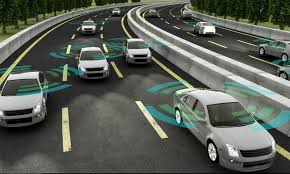
\includegraphics[scale=.20]{acar.jpeg}  \end{center} 
  \end{block}}

  
   \uncover<4->{
  \begin{block}{Robotics}
   \begin{center}  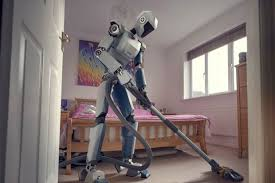
\includegraphics[scale=.20]{robot.jpeg}  \end{center} 
 \end{block}}

\column{.4\textwidth}

\uncover<3->{\begin{block}{Smart Homes}
      \begin{center}  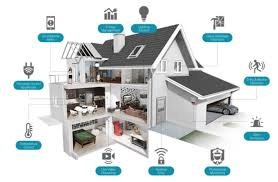
\includegraphics[scale=.20]{smarthome.jpeg}  \end{center} 
  \end{block}}

   \uncover<5->{
    \begin{block}{Chat Bots}
     \begin{center}  
\includegraphics[scale=.20]{chatbot.jpeg}  \end{center} 
   \end{block}}

  \end{columns}

  
   \uncover<6>{
    \begin{block}{}
      \begin{center} ...and many more ...
      %  : from finance market bots to personal devices like insullin controllers
     % \end{center}
   % \end{block}}
  
  % \uncover<6>{
  %  \begin{block}{}
  %    \begin{center}
        AI is in urgent need of verification: safety, security, robustness to changing conditions and adversarial attacks, ...
				\end{center}
    \end{block}}

  \end{frame}
	
	\begin{frame}
  \frametitle{Neural Nets in Massive use}
 

    
 \begin{columns}
   \column{.4\textwidth}

   
    \begin{center}
      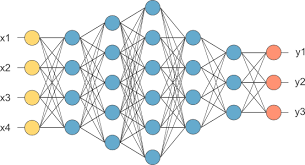
\includegraphics[scale=0.3]{NN}
    \end{center}  

\begin{block}{Used for:}

 \begin{itemize}
  \item computer vision 
  \item speech recognition
  \item  (big) data processing
    \item ...
    \end{itemize}

  
\end{block}





\column{.4\textwidth}

 
\begin{block}{In:}
 
\begin{itemize}
\item autonomous cars
\item robots
\item airport security
  \item financial applications
\item $\ldots$
\item Alexa
\item Google bot on mobile phones
\item image recognising apps 
\end{itemize}

  \end{block}


 \end{columns}
    
\end{frame}

\begin{frame}
\frametitle{Research topics in Neural nets}
\begin{block}{Weaknesses of Neural nets}
\begin{itemize}
	\item not easily conceptualised (\alert{lack of explainability})
	\item prone to error
	\item prone to adversarial attack
\end{itemize}
\end{block}
\end{frame}



\begin{frame}
\frametitle{Problems with Neural Net Verification}



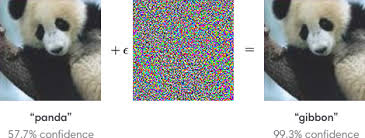
\includegraphics[width=9cm]{panda}
\pause

\begin{itemize}
	\item Verification needed: many issues with safety (autonomous devices, cars), security (adversarial attacks)
	\item Problem: -- even to state verification conditions!
	\item Current methods: Neurons to Logic (\emph{\'a la} McCulloch and Pitts), Automated Theorem proving, SMT solvers
\end{itemize}
%\pause
%\alert{I will give a short intro to verification of NN in python next week} (non-compulsory)
\end{frame}

  \begin{frame}
  \frametitle{The literature splits}
       \begin{block}{There are two groups of properties we may want to verify:}
\begin{itemize}
\item  \alert{General (concerning properties of learning algorithms):} e.g. how well does the learning algorithm perform? do trained  neural networks generalise well?\\

    {\scriptsize
 \begin{thebibliography}{99}
 \beamertemplatearticlebibitems
\bibitem{1}{A. Bagnall and G. Stewart. Certifying the True Error: Machine Learning in Coq with Verified Generalisation Guarantees. AAAI 2019.}
  \bibitem{4}{A. Bahrami, E. de Maria and A.Felty. Modelling and Verifying Dynamic Properties of Biological Neural Networks in Coq. 2018.}
 \end{thebibliography}}
  
          \pause
        \item  \alert{Specific to applications (concerning neural network deployment):} given this trained neural network, is it robust to adversarial attacks?

    {\scriptsize
 \begin{thebibliography}{99}
 \beamertemplatearticlebibitems
\bibitem{2}{X. Huang and M. Kwiatkowska and S. Wang and M. Wu. Safety Verification of Deep Neural Networks. CAV (1) 2017: 3-29}
\bibitem{3}{G. Singh, T. Gehr, M. Puschel, M. T. Vechev:
An abstract domain for certifying neural networks. PACMPL 3(POPL): 41:1-41:30 (2019)}
  \end{thebibliography}}
          
          \end{itemize}
          \end{block}
          \end{frame}


\section{Z3 API in Python}
	
	\begin{frame}[fragile]
      \frametitle{Robustness Verification scenario}
			\begin{block}{SMT Solvers}
			
			\begin{itemize}
				\item Widely used in verification \pause
				\item Z3 is one of the most popular \pause
				\item There is Z3 API in Python \pause
				\item It is often used in NN verification \pause
			\end{itemize}
			\end{block}
			\alert{Example of Z3 Python API at work:}
			\begin{verbatim}
			from z3 import *

x = Int('x')
y = Int('y')
solve(x > 2, y < 10, x + 2*y == 7)

			\end{verbatim}
			\pause
			
			\begin{itemize}
                        \item will find all solutions or say that no exist.
                          \item \alert{DEMO of Z3 in Python}
			\end{itemize}
                      \end{frame}

\begin{frame}
  \frametitle{Quantifiers and Theories}
  ... Z3 Demo in Python
\end{frame}

\section{Example of Z3 API in use: Verification of Perceptron}

\begin{frame}
\frametitle{Simple example: Perceptron}

Neural nets doing logic [McCulloch and Pitts, 1943]:

\begin{center}
\includegraphics[width=0.7\textwidth]{xor}
\end{center}
\begin{center}
\begin{tabular}{|ll |l |l |l|}
%\multicolumn{6}{l}{\alert{Training Examples:}}\\
\hline
 A & B & A \alert{and} B &  A \alert{or} B & A \alert{xor} B \\ \hline
true & true & true & true & false \\
true & false & false & true & true \\
false & true & false & true & true \\
false & false & false & false & false \\
\hline 
\end{tabular}
\end{center}

\end{frame}


\begin{frame}
\frametitle{Perceptron for \alert{and}}


$$\xymatrix@R=0.5pc@C=0pc{
&*\txt{$A$}\ar[rrrr]&&&&*\txt{\alert{$w_{A}$}}\ar[rrrrd]&&&&&&&&\\
&*\txt{$B$}\ar[rrrr]&&&&*\txt{\alert{$w_{B}$}}\ar[rrrr]&&&&*+++[o][F]{\alert{and}}\ar[rrr]&&&*\txt{?}&\\
} $$

Input features and target features:

\begin{center}
\begin{tabular}{|ll |l |}
%\multicolumn{6}{l}{\alert{Training Examples:}}\\
\hline
 A & B & A \alert{and} B  \\ \hline
true & true & true  \\
true & false & false \\
false & true & false \\
false & false & false \\
\hline 
\end{tabular}
\end{center}
\pause

Now train the network: will it be able to \alert{learn} the correct (linear) function $\theta + w_A \times A + w_B \times B$ to simulate \alert{and}? 

\pause 

 e.g. $-0.9 + 0.5 \times A + 0.5 \times B$

\end{frame}

                      
	
		\begin{frame}[fragile]
      \frametitle{General motivation}
			
			General motivation is to make  the solver:
			
			
			\begin{itemize}
				\item solve constraints like:			
			\begin{verbatim}
	(forall m n. ( (m >=. 0.5R) /\ (n >=. 0.5R)) ==> 
	    (nextoutput perceptron [m ; n]) == 1)
	\end{verbatim}
	\pause \item ... that is, to guarantee correctness of inputs for certain small range of deviations from the well-classified input
	\pause \item If the new input does not fall within the set constraints, it cannot be guaranteed to be robust to attack
	\pause \item Imagine an autonomous car passing control to a human if it cannot guarantee robust recognition of some crucial street signs. 

			\end{itemize}
	\end{frame}
	
	\begin{frame}[fragile]
      \frametitle{Simple Robustness Verification scenario}
      \begin{itemize}
      \item Implement my Perceptron in Python \pause
      \item Prove it is robust for class 1: \pause
        \begin{itemize}
      \item Define its robustness region: e.g. when input array contains real values in 
        the region $\epsilon$ given (say) by some Eucledian distance  from our ideal input $[1,1]$ \pause
      \item define a step function (``the ladder'') to generate a finite number of reals in this region (otherwise Z3 will not terminate) \pause
      \item Prove the ladder is ``covering'' (using pen and paper) \pause
      \item  Take the set of input generated by Z3, run them through the Perceptron \pause
        \item No mis-classification? -- I have proven my network robust for output $1$, region $\epsilon$ and the ladder.
\end{itemize}
\end{itemize}


%\pause

%\begin{block}{Problems}
%  \begin{itemize}
%  \item No direct access to Perceptron implementation from Z3
%  \item Fragility of type conversion between Python and Z3
%    \item Either ``Testing flavour'' or manual proofs are needed
%    \end{itemize}
%  \end{block}

      \end{frame}
	

      \begin{frame}
        \frametitle{Demo}
        ... of how this methodology is reaslised in Python with Z3.
        \end{frame}
      

\end{document}
